% Copyright (c) 2008, João Henrique Ferreira de Freitas
% All rights reserved.
% 
% Redistribution and use in source and binary forms, with or without modification,
% are permitted provided that the following conditions are met:
% 
%     * Redistributions of source code must retain the above copyright notice,
%       this list of conditions and the following disclaimer.
%     * Redistributions in binary form must reproduce the above copyright notice,
%       this list of conditions and the following disclaimer in the documentation and/or 
%       other materials provided with the distribution.
%     * Neither the name of the <ORGANIZATION> nor the names of its contributors may
%       be used to endorse or promote products derived from this software without 
%       specific prior written permission.
% 
% THIS SOFTWARE IS PROVIDED BY THE COPYRIGHT HOLDERS AND CONTRIBUTORS "AS IS" AND ANY 
% EXPRESS OR IMPLIED WARRANTIES, INCLUDING, BUT NOT LIMITED TO, THE IMPLIED WARRANTIES
% OF MERCHANTABILITY AND FITNESS FOR A PARTICULAR PURPOSE ARE DISCLAIMED. IN NO EVENT
% SHALL THE COPYRIGHT OWNER OR CONTRIBUTORS BE LIABLE FOR ANY DIRECT, INDIRECT, INCIDENTAL,
% SPECIAL, EXEMPLARY, OR CONSEQUENTIAL DAMAGES (INCLUDING, BUT NOT LIMITED TO, PROCUREMENT
% OF SUBSTITUTE GOODS OR SERVICES; LOSS OF USE, DATA, OR PROFITS; OR BUSINESS INTERRUPTION)
% HOWEVER CAUSED AND ON ANY THEORY OF LIABILITY, WHETHER IN CONTRACT, STRICT LIABILITY,
% OR TORT (INCLUDING NEGLIGENCE OR OTHERWISE) ARISING IN ANY WAY OUT OF THE USE OF THIS
% SOFTWARE, EVEN IF ADVISED OF THE POSSIBILITY OF SUCH DAMAGE.
% 
% $Id$

\mode<presentation>
{
  \usetheme{Warsaw}
  %\setbeamercovered{transparent}
}

\usepackage[brazil]{babel}    % dá suporte para os termos na língua portuguesa do Brasil
\usepackage[latin1,utf8]{inputenc}
% \usepackage{subfigure}         % figuras e tabelas lado a lado
\usepackage{graphics}          % figuras gráficas
% \usepackage{color}             % para letras e caixas coloridas
% \usepackage{hyperref}          % faz funcionar o \hipersetup
% \usepackage{url}

\usepackage{times}
\usepackage[T1]{fontenc}
\usepackage{pgf}

\title[Evidenciação de processo para contribuição em SL/CA]{Evidenciação Empírica de um Processo para Contribuição em Projetos de Software Livre e Código Aberto}

\author{João Henrique Ferreira de Freitas\inst{1}}
\date{\today}

\institute[UFLA] % (optional, but mostly needed)
{
  \inst{1}%
  Pós Graduação em Desenvolvimento de Software\\
  Universidade Federal de Lavras
}

\date[Encontro UFLA 2008] % (optional, should be abbreviation of conference name)
{Encontro Técnico UFLA, 2008}

\mode<presentation>{\subject{Processos de Software}}

\AtBeginSubsection[]
{
}

\begin{document}

\begin{frame}
  \titlepage
\end{frame}

% Structuring a talk is a difficult task and the following structure
% may not be suitable. Here are some rules that apply for this
% solution: 

% - Exactly two or three sections (other than the summary).
% - At *most* three subsections per section.
% - Talk about 30s to 2min per frame. So there should be between about
%   15 and 30 frames, all told.

% - A conference audience is likely to know very little of what you
%   are going to talk about. So *simplify*!
% - In a 20min talk, getting the main ideas across is hard
%   enough. Leave out details, even if it means being less precise than
%   you think necessary.
% - If you omit details that are vital to the proof/implementation,
%   just say so once. Everybody will be happy with that.

% 3 min

\section{Introdução}

\subsection{Objetivos}

\begin{frame}{Propósitos gerais}
 \begin{itemize}
  \item <1-> Relatar, através de uma experiência, um processo e prática para a contribuição e melhoramento em SL/CA;
  \item <2- | alert@2> Responder a pergunta principal do trabalho: Como colaborar efetivamente?
  \item <3-> Três projetos iniciais: 
     \begin{itemize}
       \item <4- > Tikiwiki;
       \item <5-> Pfsense;
       \item <6-> Bacula;
     \end{itemize}  
   \item <7-> Apenas um escolhido para as experiências.
 \end{itemize}
\end{frame}

\begin{frame}{Propósitos pessoais}
 \begin{itemize}
 \item <1-> Aumentar o conhecimento em desenvolvimento de software;
 \item <2-> Colaborar com o desenvolvimento de um produto internacional;
 \item <3-> Implementar e resolver necessidades referentes as funcionalidades desejadas do software escolhido.
 \end{itemize}
\end{frame}

\subsection{Posicionamentos}
 \begin{frame}{Definição de termos}
  \begin{description}
   \item [Colaboração] submissão de patchs que são definidos como mudanças, consertos ou melhoramentos contendo código fonte, documentação e processos;
   \item [Projeto de SL/CA] é uma organização virtual centrada em torno de um código fonte, com participação espontânea e variável de pessoas.
  \end{description}
 \end{frame}

 \begin{frame}{Ponto de observações}
   %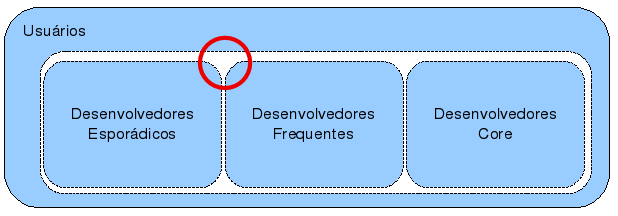
\includegraphics{../../doc/diagramas/equipe}
   \pgfdeclareimage[height=3cm]{equipe}{../../doc/diagramas/equipe}
   \begin{center}
      \pgfuseimage{equipe}
   \end{center}
 \end{frame}

\subsection{Objetivos práticos}
  \begin{frame}{Objetivos práticos} 
    \begin{itemize}
      \item Contribuir implementando um novo recurso de interfaceamento com SGBDs para o projeto escolhido;
      \item Referenciado no trabalho como patch libdbi;
      \item Atravez da experiência, vivenciamos e capturamos o processo utilizado durante o desenvolvimento do patch.
    \end{itemize}
  \end{frame}

  \begin{frame}{Projeto de SL/CA escolhido}
  Projeto Bacula (www.bacula.org) devido aos seguintes fatores:
    \begin{itemize}
    \item Tempo de atividade: 10 anos;
    \item Segmento da aplicação: meio corporativo e infraestrutura;
    \item Documentação: completa, nivelada e atualizada;
    \item Comunidade formada: usuário, desenvolvedores, empresas;
    \item Comprometimento.
    \end{itemize}
    \pgfdeclareimage[height=0.7cm]{bacula}{../../doc/figuras/bacu_logo}
    \begin{center}
        \pgfuseimage{bacula}
    \end{center}
  \end{frame}

  \begin{frame}{Arquitetura geral do Bacula}
    \pgfdeclareimage[width=8cm,height=6.8cm]{bacula_arquitetura}{../../doc/diagramas/bacula_arquitetura}
    \begin{center}
      \pgfuseimage{bacula_arquitetura}
    \end{center}
  \end{frame}

  \begin{frame}{Antes do patch libdbi}
    \begin{columns}
      \begin{column}{5cm}
        \begin{itemize}
          \item <1> Somente três SGBDs suportados (Mysql, Postgresql, Sqlite);
          \item <2> Modular mas dependente de implementação e API de cada SGBD;
          \item <3> Três códigos distintos para manter.
        \end{itemize}
      \end{column}
      \begin{column}{5cm}
        \pgfdeclareimage[width=5cm]{antes}{../../doc/diagramas/bacula_catalog}
        \pgfuseimage{antes}
      \end{column}
    \end{columns}
  \end{frame}

  \begin{frame}{Após o patch libdbi}
    \begin{columns}
      \begin{column}{5cm}
        \begin{itemize}
          \item <1> Vários tipos de SGBDs podem ser suportados;
          \item <2> Modular sem dependência de implementação e API;
          \item <3> Ponto único para manutenção e refactoting.
        \end{itemize}
      \end{column}
      \begin{column}{5cm}
        \pgfdeclareimage[width=5cm]{depois}{../../doc/diagramas/bacula_libdbicatalog}
        \pgfuseimage{depois}
      \end{column}
    \end{columns}
  \end{frame}

\section{Exposição da Experiência}

\subsection{Classificação}
\begin{frame}{Coleta de dados}
Buscas no \emph{hyperespaço}, Internet: 
  \begin{itemize}
    \item <1-> Websites;
    \item <2-> Listas de e-mail públicas;
    \item <3-> IRC chats;
    \item <4-> Artefatos no repositório de controle de versão;
    \item <5-> Documentação oficial do projeto.
  \end{itemize}
\end{frame}

\begin{frame}{Taxionomia}
Classificação dos artefatos levantados em três grupos:
  \begin{itemize}
  \item <1-> Estrutural, como são desenvolvidos e organizados;
  \item <2-> Conteúdo, tipos de artefatos e conteúdos;
  \item <3-> Padrões de utilização, interação do usuário, desenvolvedores, atualização.
  \end{itemize}
\end{frame}

\begin{frame}{Taxionomia, site do projeto}
  \pgfdeclareimage[width=8cm]{website_main}{../../doc/websites/bacula_website_main}
  \pgfuseimage{website_main}
\end{frame}
\begin{frame}{Taxionomia, projetos ativos}
  \pgfdeclareimage[width=8cm]{website_projects}{../../doc/websites/bacula_website_projects}
  \pgfuseimage{website_projects}
\end{frame}
\begin{frame}{Taxionomia, documentação}
  \pgfdeclareimage[width=8cm]{website_docs}{../../doc/websites/bacula_website_docs}
  \pgfuseimage{website_docs}
\end{frame}
\begin{frame}{Taxionomia, bugtrack}
  \pgfdeclareimage[width=8cm]{website_bugs}{../../doc/websites/bacula_website_bugs}
  \pgfuseimage{website_bugs}
\end{frame}
\begin{frame}{Taxionomia, guia de desenvolvimento}
  \pgfdeclareimage[width=8cm]{bacula_develsguide}{../../doc/websites/bacula_develsguide}
  \pgfuseimage{bacula_develsguide}
\end{frame}
\begin{frame}{Taxionomia, testes de regressão}
  \pgfdeclareimage[width=8cm]{bacula_regress}{../../doc/websites/bacula_regress}
  \pgfuseimage{bacula_regress}
\end{frame}
\begin{frame}{Taxionomia, análise dos testes}  
  \pgfdeclareimage[width=8cm]{bacula_dashboard2}{../../doc/websites/dashboard2}
  \pgfuseimage{bacula_dashboard2}
\end{frame}
\begin{frame}{Taxionomia, listas de discussão}
  \pgfdeclareimage[width=8cm]{bacula_gmane}{../../doc/websites/gmane_bacula_lists}
  \pgfuseimage{bacula_gmane}
\end{frame}
\begin{frame}{Taxionomia, threads da lista}
  \pgfdeclareimage[width=8cm]{bacula_gmane_thread}{../../doc/websites/bacula_develthreads}
  \pgfuseimage{bacula_gmane_thread}
\end{frame}
\begin{frame}{Taxionomia, resumo}
  \begin{center}
    \pgfdeclareimage[width=8cm]{maping}{../../doc/diagramas/maping}
    \pgfuseimage{maping}
  \end{center}
\end{frame}

\subsection{Ciclo de desenvolvimento}
\begin{frame}{Desenvolvimento}
  \begin{columns}
    \begin{column}{5cm}
      \begin{itemize}
      \item <1- | alert@1> Utilizado uma exploração arquitetural do XP;
      \item <2- | alert@2> Utilizado um modelo de programação exploratória;
      \item <3- | alert@3> Testes de regressão para validações, sempre.
      \end{itemize}
    \end{column}
    \begin{column}{5cm}
      \begin{itemize}
        \item <1> Testar;
        \item <1> Documentar;
        \item <1> Feedback;
        \item <1> Explorar;
        \item <1> Analisar.
      \end{itemize}
      \pgfdeclareimage[width=5cm]{exploracao}{../../doc/diagramas/programacao_exploratoria}
      \pgfuseimage{exploracao}<2>
    \end{column}
  \end{columns}
\end{frame}

\begin{frame}{Dia a dia de trabalho}
  \begin{columns}
    \begin{column}{5cm}
      \begin{itemize}
        \item Implementação
      \end{itemize}  
    \end{column}
      \begin{column}{5cm}
        \pgfdeclareimage[width=5cm]{resolucao1}{../../doc/diagramas/resolucao_problemas_1}
        \pgfuseimage{resolucao1}
      \end{column}
  \end{columns}
\end{frame}

\begin{frame}{Dia a dia de trabalho}
  \begin{columns}
    \begin{column}{5cm}
      \begin{itemize}
        \item Testes
      \end{itemize}  
    \end{column}
      \begin{column}{5cm}
        \pgfdeclareimage[width=5cm]{resolucao2}{../../doc/diagramas/resolucao_problemas_2}
        \pgfuseimage{resolucao2}
      \end{column}
  \end{columns}
\end{frame}

\begin{frame}{Dia a dia de trabalho}
  \begin{columns}
    \begin{column}{5cm}
      \begin{itemize}
        \item Análise
      \end{itemize}  
    \end{column}
      \begin{column}{5cm}
        \pgfdeclareimage[width=5cm]{resolucao3}{../../doc/diagramas/resolucao_problemas_3}
        \pgfuseimage{resolucao3}
      \end{column}
  \end{columns}
\end{frame}

\begin{frame}{Dia a dia de trabalho}
  \begin{columns}
    \begin{column}{5cm}
      \begin{itemize}
        \item Discussões
      \end{itemize}  
    \end{column}
      \begin{column}{5cm}        
        \pgfdeclareimage[width=5cm]{resolucao4}{../../doc/diagramas/resolucao_problemas_4}
        \pgfuseimage{resolucao4}
      \end{column}
  \end{columns}
\end{frame}

\begin{frame}{Dia a dia de trabalho}
  \begin{columns}
    \begin{column}{5cm}
      \begin{itemize}
        \item Submissão
      \end{itemize}  
    \end{column}
      \begin{column}{5cm}
        \pgfdeclareimage[width=5cm]{resolucao5}{../../doc/diagramas/resolucao_problemas_5}
        \pgfuseimage{resolucao5}
      \end{column}
  \end{columns}
\end{frame}

\subsection{Timeline das atividades}

  \begin{frame}{Timeline}
    \pgfdeclareimage[width=12cm]{timeline}{../../doc/planilhas/datas_do_desenvolvimento}
    \pgfuseimage{timeline}
  \end{frame}


% 1 min
\section{Aprendizados}
\begin{frame}{Aprendizado: Técnico}
  \begin{itemize}
  \item Aprofundamento em C/C++;
  \item Atenção a refactoring;
  \item Leitura de código fonte aprimorado;
  \item Entendimento do domínio do problema;
  \item Conhecimento em ferramentas de suporte (autoconf, automake, libtool, Makefiles).
  \end{itemize}
\end{frame}

\begin{frame}{Aprendizado: Engenharia de Software}
Na prática:
  \begin{itemize}
  \item Testes de regressão;
  \item Construir para verificação;
  \item Aderência a padrões;
  \item Modularidade;
  \end{itemize}
\end{frame}

\begin{frame}{Aprendizado: Pessoal}
  \begin{itemize}
  \item Escrita e leitura em inglês; 
  \item Exposição de idéias em inglês;
  \item Diálogos constantes com pessoas de outros países.
  \end{itemize}
\end{frame}

% 1min

\section{Conclusão}

\begin{frame}{Processo geral de contribuição}
 \begin{enumerate}
    \item <1-> Alguém reporta um bug ou solicita uma nova funcionalidade;
    \item <2-> O item se torna prioridade, muitos usuários comentam, endoçam;
    \item <3-> Há uma discussão sobre o item mais aprofundada;
    \item <4-> Alguém posta um patch, levantando uma incerteza sobre o mesmo; 
    \item <5-> Desenvolvedores testam e comentam o patch, caso ele resolva o problema;
    \item <6-> O patch é revisto e formalmente testado;
    \item <7-> Quando o patch é considerado aceito, ele é integrado e liberado na próxima versão.
  \end{enumerate}
\end{frame}

  \begin{frame}{Conclusões do Trabalho}
    \begin{itemize} 
      \item <1-> Cada projeto de SL/CA estabelece seus próprios meios. Mas existem similaridades entre eles:
      \begin{itemize}
        \item Discussões em listas de email públicas;
        \item Gerenciamento do código fonte e configuração;
        \item Desenvolvimento próximo do usuário final.
      \end{itemize}
      \item <2-> Os portais dos projetos apresentam muito sobre suas características e formas de organização;
      \item <3-> Existe um caminho pré suposto no qual o usuário necessita seguir para colaborar efetivamente.
    \end{itemize}
  \end{frame}
  \begin{frame}{Conclusões Pessoais}
    \begin{itemize}
      \item <1-> As contribuições são aceitas em projetos de SL/CA. Mas é necessário bom senso, diálogo intenso, carisma, entendimento do problema e pró-atividade;
      \item <2-> Trabalhe sempre para não quebrar o código já funcional e com certeza a sua contribuição será aceita.
    \end{itemize}
  \end{frame}

\section{Trabalhos Futuros}
  \begin{frame}{Dentro das comunidades de SL/CA}
    \begin{itemize}
      \item Suporte e manutenção do patch libdbi para o projeto Bacula;
      \item Contribuições no framework libdbi: casos de testes, novos drivers, profiling e benchmarks;
      \item Continuar pesquisas relacionado a busca de padrões em projetos de SL/CA.
    \end{itemize}
  \end{frame}

  \begin{frame}{Contato}
    \begin{center}
     \begin{Large}
João Henrique Ferreira de Freitas \\
joaohf@gmail.com \\ 
\vspace{1cm}
http://joaohff.pbwiki.com \\
http://joaohf.livejournal.com
      \end{Large}
    \end{center}
  \end{frame}

\end{document}
